% Overleaf-ready visual appendix for Week 1-4 presentation/report
\documentclass[11pt]{article}
\usepackage[margin=1in]{geometry}
\usepackage{tikz}
\usepackage{pgfplots}
\usepackage{booktabs}
\pgfplotsset{compat=1.18}
\usetikzlibrary{arrows.meta,positioning,shapes.geometric,fit}

\title{MedLens Cloud-Edge Project Visuals (Week 1-4)}
\author{}
\date{}

\begin{document}
\maketitle

\section*{1. Cloud-Edge-Device Architecture}
\begin{center}
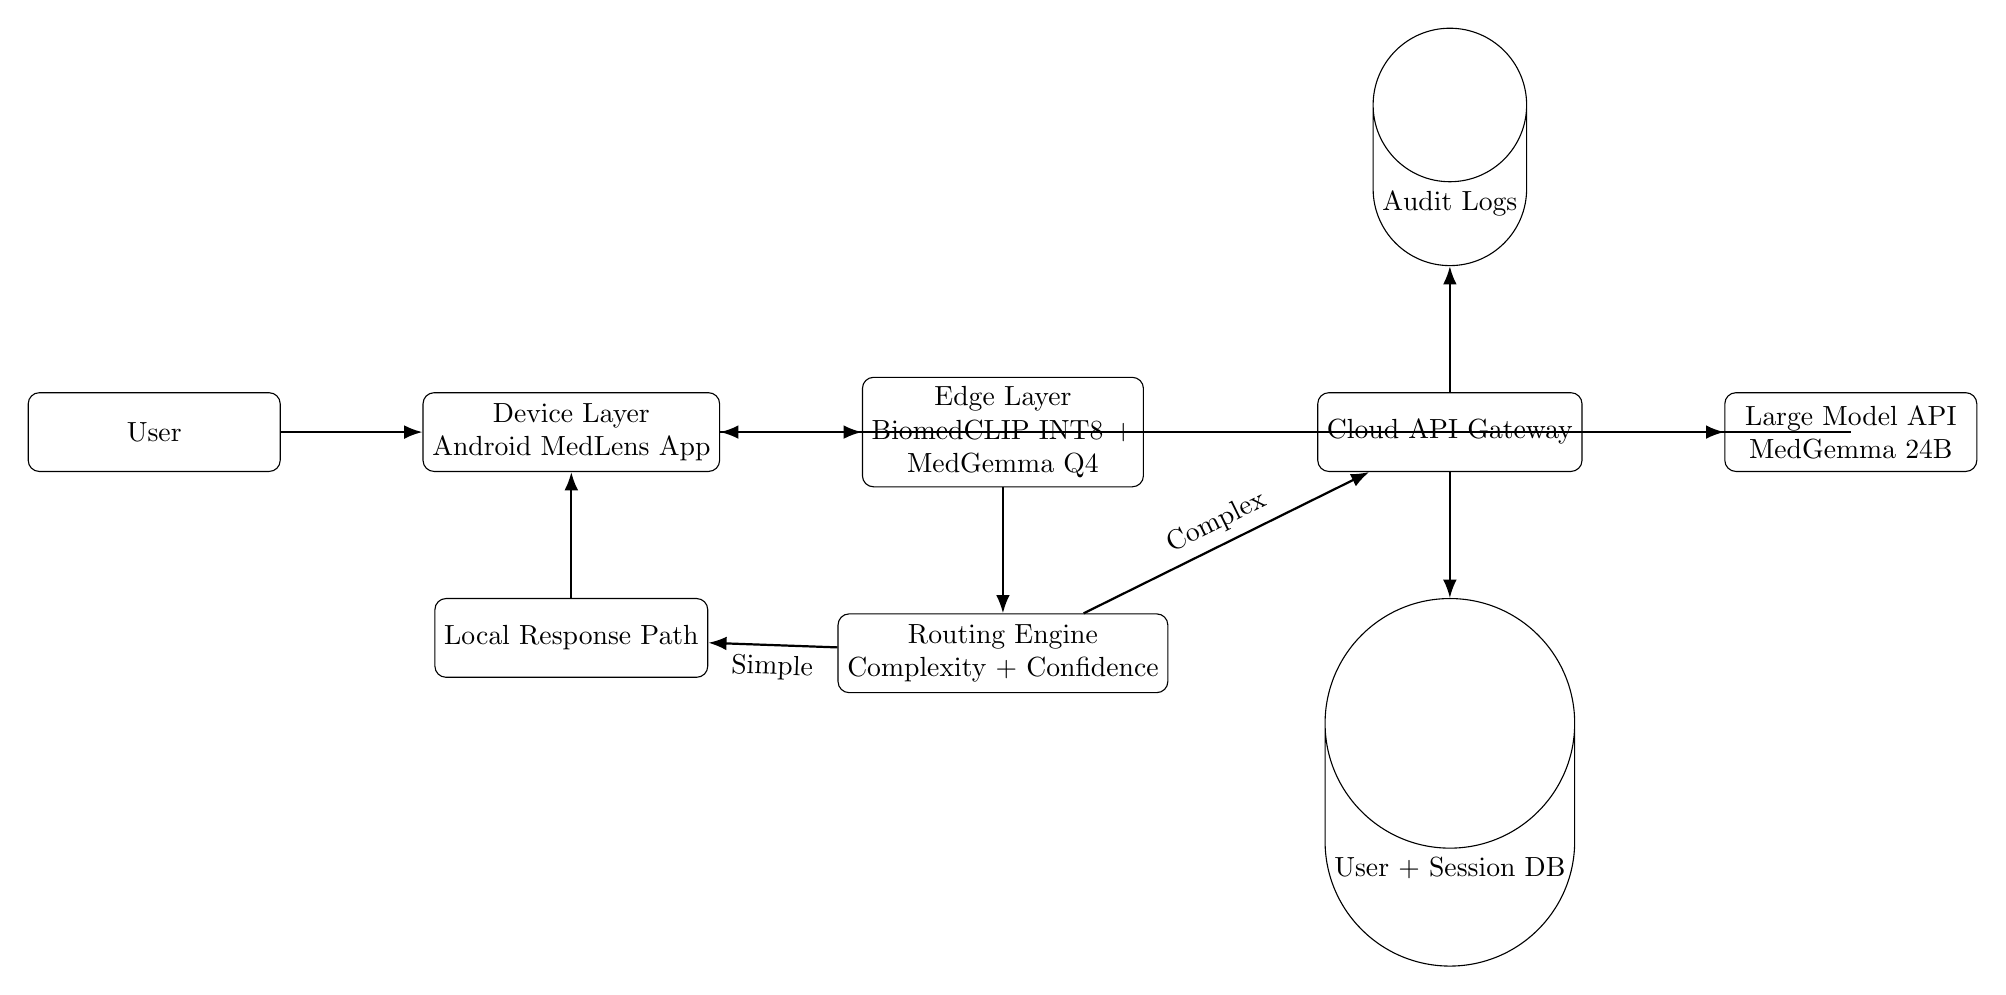
\begin{tikzpicture}[
  node distance=1.6cm and 1.8cm,
  box/.style={draw, rounded corners, align=center, minimum width=3.2cm, minimum height=1.0cm},
  data/.style={draw, cylinder, shape border rotate=90, align=center, minimum height=1.0cm, minimum width=1.7cm},
  arr/.style={-Latex, thick}
]
\node[box] (u) {User};
\node[box, right=of u] (d) {Device Layer\\Android MedLens App};
\node[box, right=of d] (e) {Edge Layer\\BiomedCLIP INT8 +\\MedGemma Q4};
\node[box, below=of e] (r) {Routing Engine\\Complexity + Confidence};
\node[box, right=2.2cm of e] (c) {Cloud API Gateway};
\node[box, right=of c] (m) {Large Model API\\MedGemma 24B};
\node[data, below=of c] (db) {User + Session DB};
\node[data, above=of c] (log) {Audit Logs};
\node[box, below=of d] (l) {Local Response Path};

\draw[arr] (u) -- (d);
\draw[arr] (d) -- (e);
\draw[arr] (e) -- (r);
\draw[arr] (r) -- node[above, sloped]{Complex} (c);
\draw[arr] (r) -- node[below, sloped]{Simple} (l);
\draw[arr] (c) -- (m);
\draw[arr] (c) -- (db);
\draw[arr] (c) -- (log);
\draw[arr] (l) -- (d);
\draw[arr] (m) |- (d);
\end{tikzpicture}
\end{center}

\section*{2. Routing Decision Flow}
\begin{center}
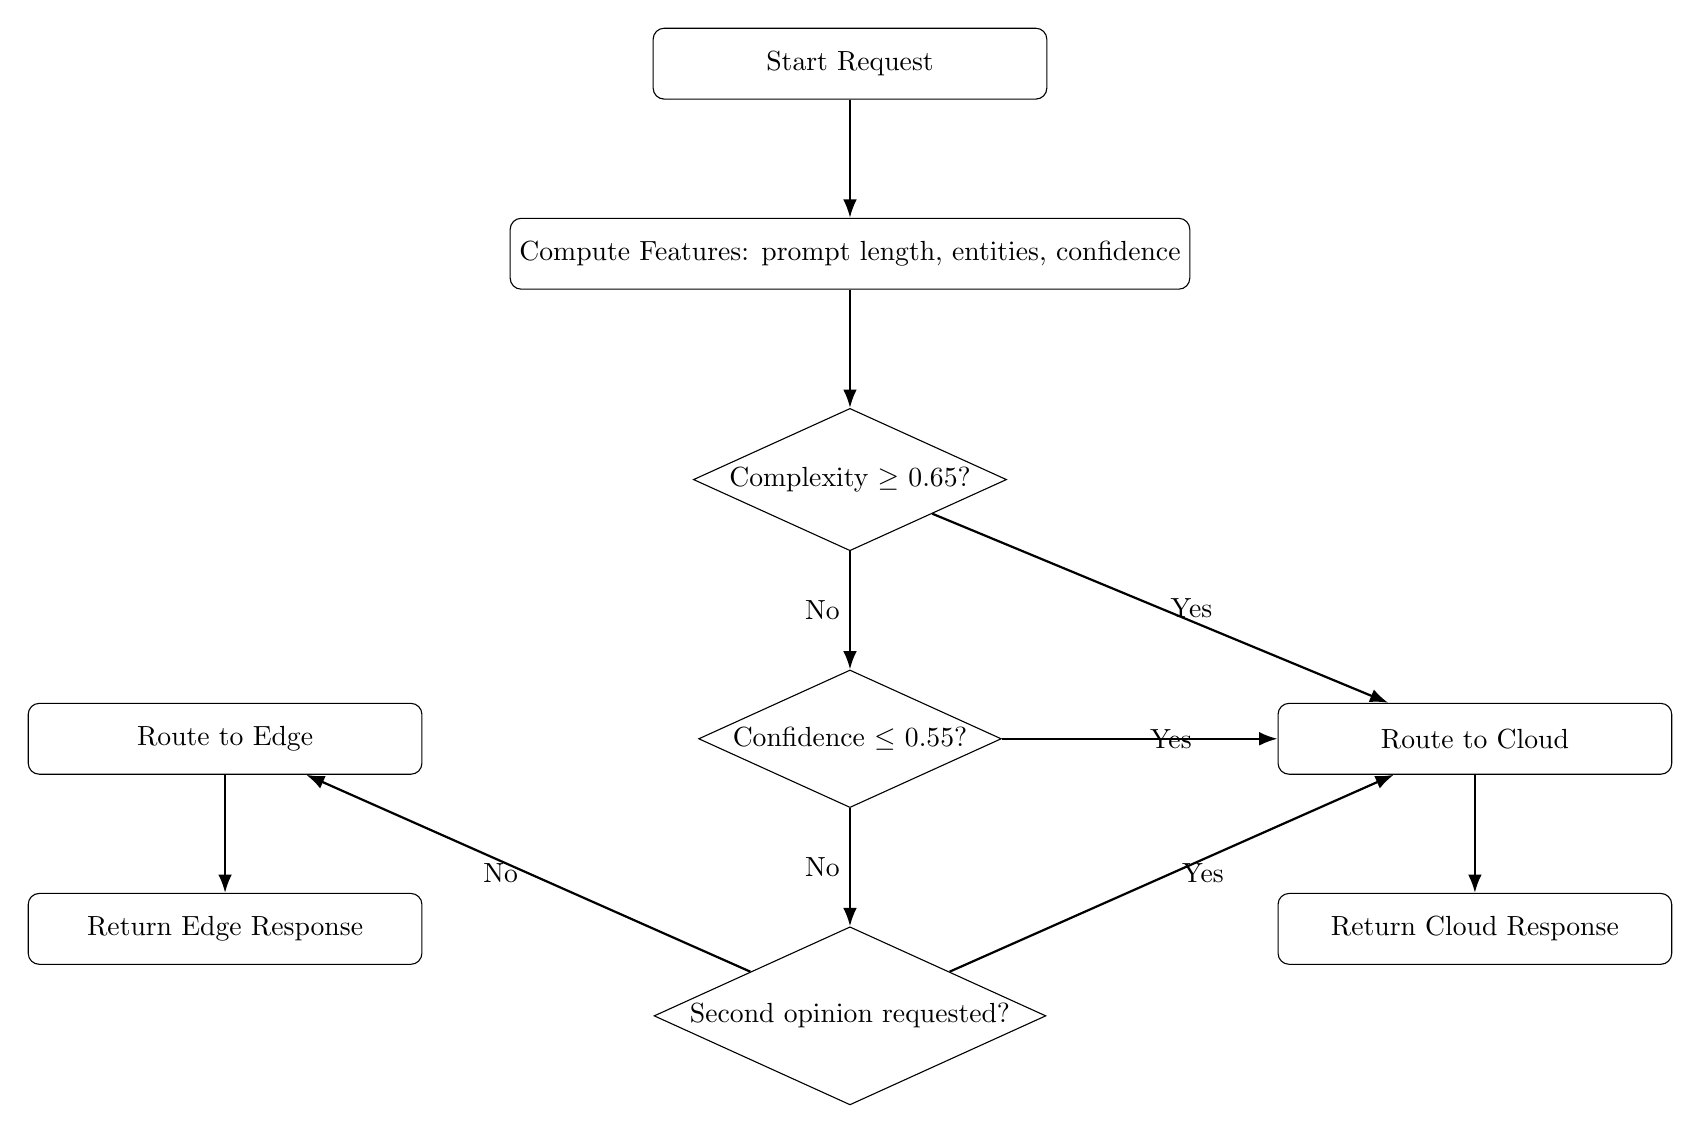
\begin{tikzpicture}[
  node distance=1.5cm,
  block/.style={draw, rounded corners, align=center, minimum width=5cm, minimum height=0.9cm},
  decision/.style={draw, diamond, aspect=2.2, align=center, inner sep=1pt},
  arr/.style={-Latex, thick}
]
\node[block] (a) {Start Request};
\node[block, below=of a] (b) {Compute Features: prompt length, entities, confidence};
\node[decision, below=of b] (c) {Complexity $\geq$ 0.65?};
\node[decision, below=of c] (d) {Confidence $\leq$ 0.55?};
\node[decision, below=of d] (e) {Second opinion requested?};
\node[block, right=3.5cm of d] (g) {Route to Cloud};
\node[block, left=3.5cm of d] (f) {Route to Edge};
\node[block, below=of f] (h) {Return Edge Response};
\node[block, below=of g] (i) {Return Cloud Response};

\draw[arr] (a) -- (b);
\draw[arr] (b) -- (c);
\draw[arr] (c) -- node[right]{Yes} (g);
\draw[arr] (c) -- node[left]{No} (d);
\draw[arr] (d) -- node[right]{Yes} (g);
\draw[arr] (d) -- node[left]{No} (e);
\draw[arr] (e) -- node[right]{Yes} (g);
\draw[arr] (e) -- node[left]{No} (f);
\draw[arr] (f) -- (h);
\draw[arr] (g) -- (i);
\end{tikzpicture}
\end{center}

\section*{3. Week 1-4 Status Chart}
\begin{center}
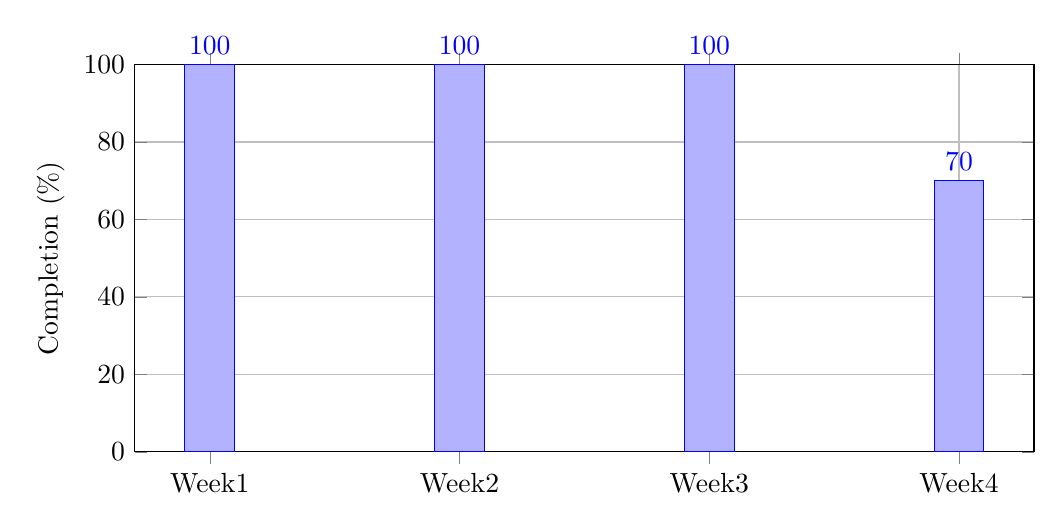
\begin{tikzpicture}
\begin{axis}[
    ybar,
    bar width=18pt,
    width=13cm,
    height=6.5cm,
    ymin=0,
    ymax=100,
    ylabel={Completion (\%)},
    symbolic x coords={Week1,Week2,Week3,Week4},
    xtick=data,
    nodes near coords,
    nodes near coords align={vertical},
    grid=major,
]
\addplot coordinates {(Week1,100) (Week2,100) (Week3,100) (Week4,70)};
\end{axis}
\end{tikzpicture}
\end{center}

\section*{4. Week 4 Cloud Service Scope}
\begin{center}
\begin{tabular}{ll}
\toprule
Service Endpoint & Purpose \\
\midrule
POST /v1/route-evaluate & Decide edge vs cloud path \\
POST /v1/qa/cloud-infer & Run large-model inference \\
POST /v1/sessions & Store session metadata \\
GET /v1/health & Service liveness for demo \\
\bottomrule
\end{tabular}
\end{center}

\end{document}
